\documentclass{article}
\usepackage[utf8]{inputenc}
\usepackage[norsk]{babel}
\usepackage{mathtools} 
\usepackage{hyperref}
\usepackage{listings} 
\usepackage{graphicx}
\begin{document}
\begin{titlepage}
\begin{center}

\vspace*{3cm}
\textsc{\Huge D2b}\\[0.7cm]
\textsc{\medium TTM4100 - Communication Services and Networks}\\[0.3cm]
\textsc{\medium TDT4140 - Software Enigneering}\\[0.3cm]
\textsc{\medium TDT4145 - Data Modeling, Databases and Database Management Systems}\\[0.3cm]
\textsc{\medium TDT4180 - Human-Computer Interaction}\\[0.3cm]

\textbf{\Large Gruppe 7:} \\[0.2cm]
\text{\Large Espen Albert, Finn Inderhaug, Kristoffer Andreas Dalby} \\
\text{\Large Christoffer B. Nysæter, Andreas Wien, Jonas André Dalseth}\\[1cm]

\today

\end{center}
\end{titlepage}



\section{Description of the prototype}
% remember to put graphs har, use \begin{figure } from wiki
\begin{figure}[h!] 
    \begin{center} 
        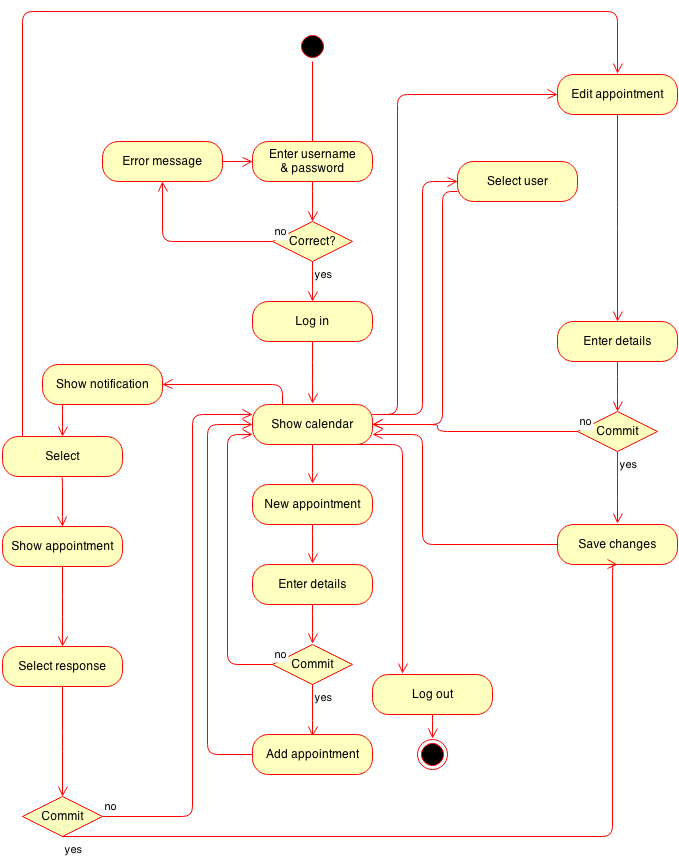
\includegraphics[width=8cm]{img/calendarStateDiagram.png}
        \caption{Calendar state diagram}
    \label{calendarstatediagram}
    \end{center}
\end{figure}

\begin{figure}[h!] 
    \begin{center} 
        \includegraphics[width=8cm]{img/IMG_5600.png}
        \caption{Log in screen}
    \label{login}
    \end{center}
\end{figure}

\begin{figure}[h!] 
    \begin{center} 
        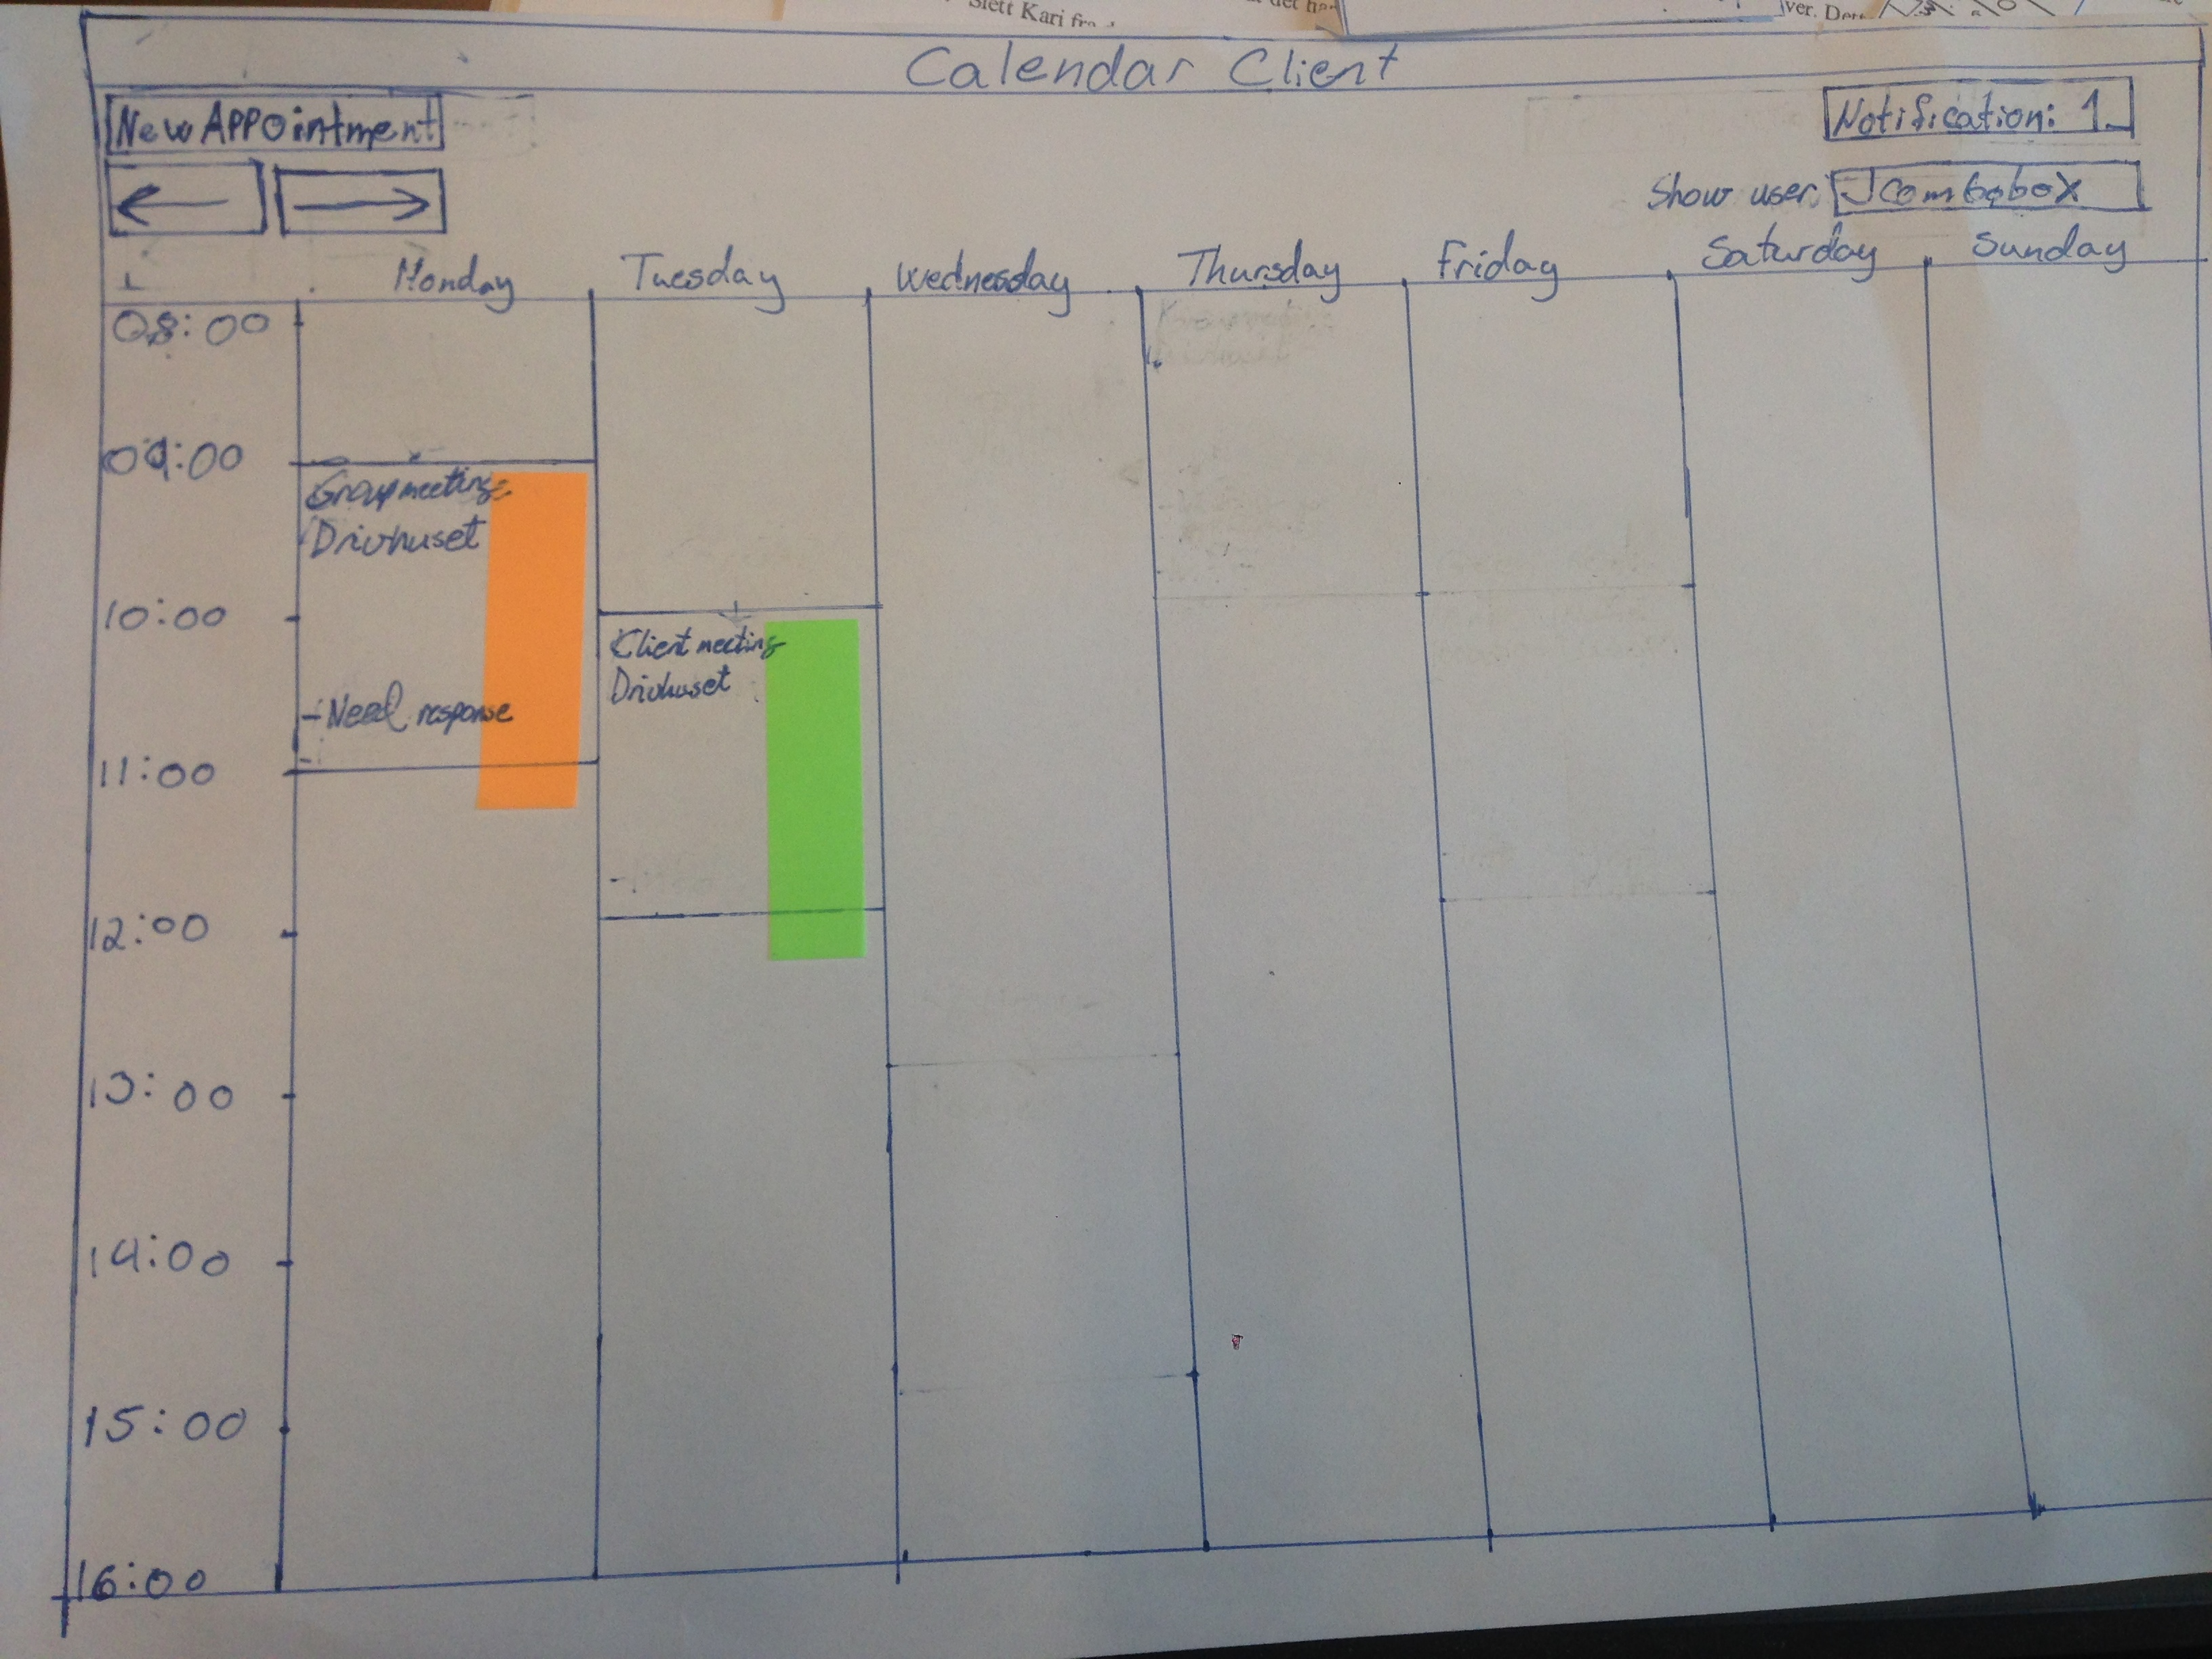
\includegraphics[width=8cm]{img/IMG_5601.JPG}
        \caption{Week view}
    \label{weekview}
    \end{center}
\end{figure}

\begin{figure}[h!] 
    \begin{center} 
        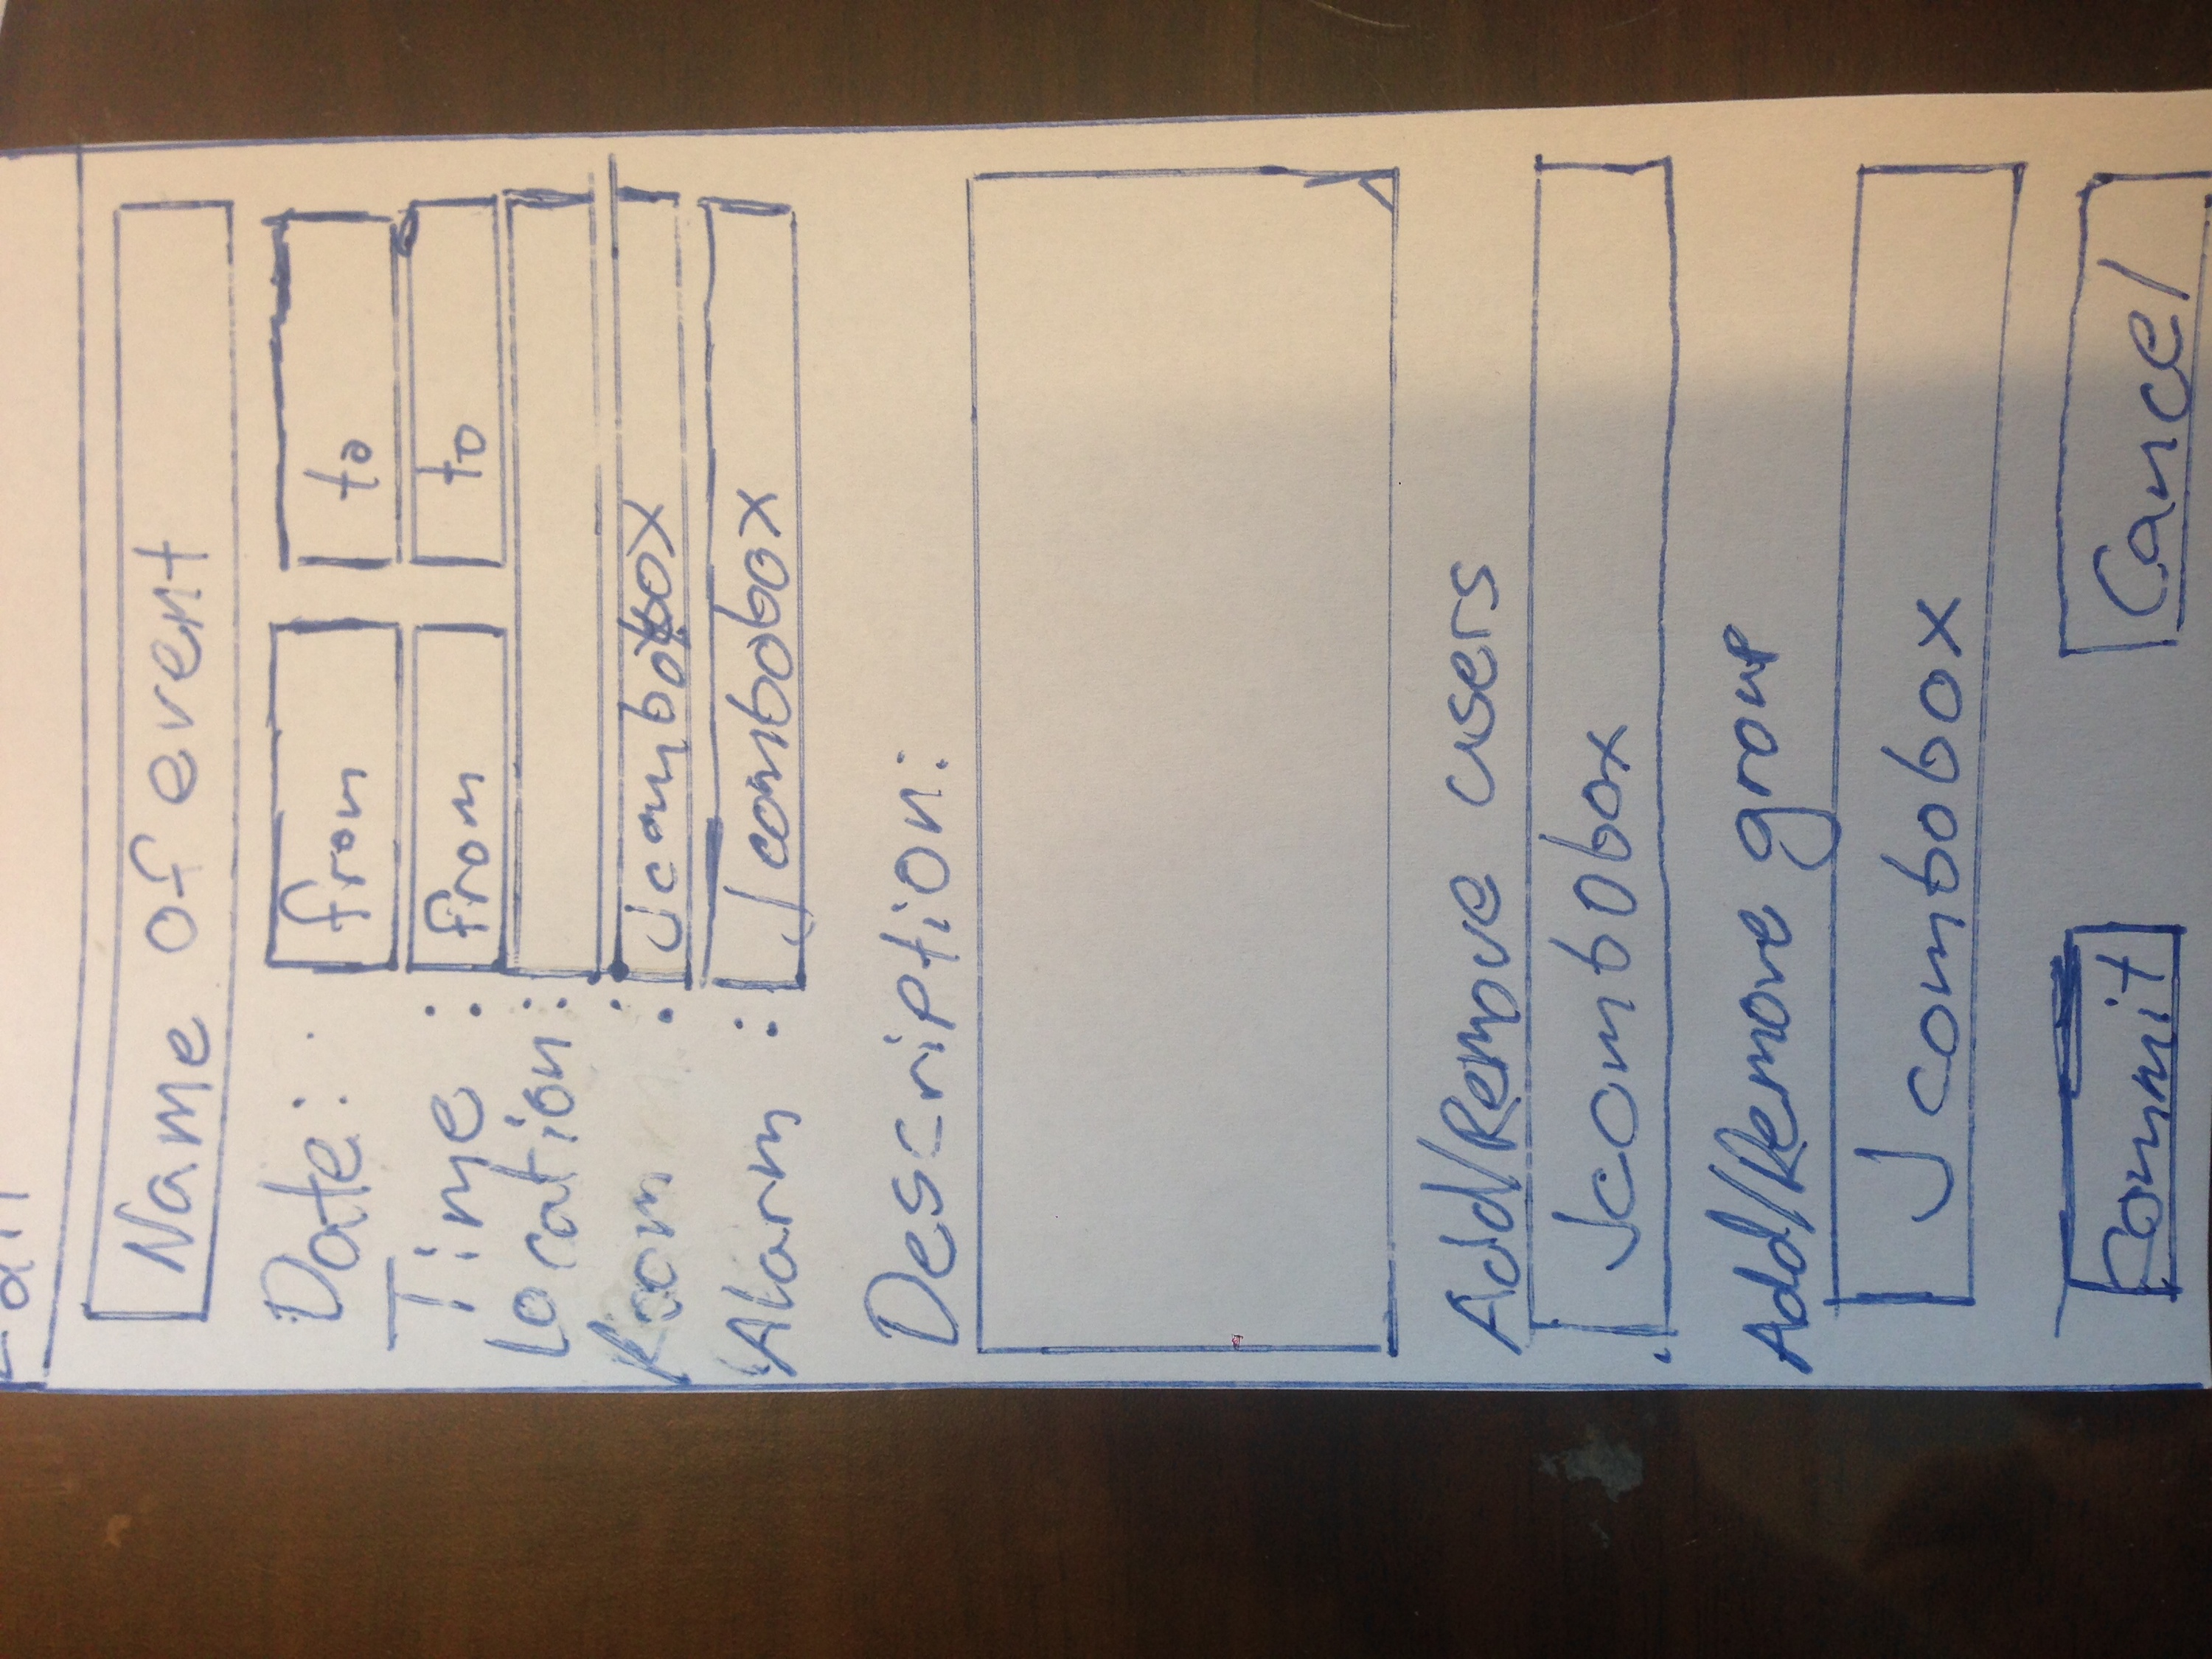
\includegraphics[width=8cm]{img/IMG_5602.JPG}
        \caption{Edit screen}
    \label{edit}
    \end{center}
\end{figure}

\begin{figure}[h!] 
    \begin{center} 
        \includegraphics[width=8cm]{img/IMG_5604.png}
        \caption{Room dropdown menu}
    \label{roomdropdown}
    \end{center}
\end{figure}


\section{The task at hand}
A usability test was performed to test the paperprototype. The tasks was as follows:
\begin{enumerate}

\item You shall invite a business connection to a meeting in your companys own meetingrooms (already registered in the system). You will invite Kari to a meeting from 12:00 - 14:00, 10. march, and you're supposed to book a meeting room through this calendar system.

\item Kari has now received a phonecall. Unfortunately she have to go to another more imortant meeting at the time you invited her. You will now be Kari and decline the appointment you were invited to first.

\item You're yourself again, and you have received a notification. Check this.

\item Delete Kari from this meeting and and Sindre instead.

\item Yor businessconnection calls you, and tell you he's one hour late. Change this in the appointment in the calendar.
\end{enumerate}


Ole Halvor Dahl






\section{The test with student assistant}
\subsection{Roles}
\begin{itemize}
\item Testleader: Jonas André Dalseth and Andreas Wien
\item Observers: Jonas André Dalseth, Finn Inderby, Espen Albert
\item Wizard Of Oz: Jonas André Dalseth og Andreas Wien
\item Tester: Fredrik Winther Dahl
\end{itemize}

\subsection{Exectution}
The test with the student assistant wasn't very organized. First we thought we was just supposed to show him the paper model, so we didn't have any routines. Everybody on the group guided him through different scenarios, and we hadn't made any before we met him. After the test we asked him to fill out the SUS scheme and asked him what he thought about the system. We learned a lot about talking to him, and he told us how we should do it when we tested with the other group. 
\section{The test with other group}
\subsection{Roles}
\begin{itemize}
\item Testleader: Jonas André Dalseth
\item Wizard of Oz: Andreas Wien
\item Observers: Finn Inderhaug, Kristoffer Dalby
\item Tester: Ole Halvor Dahl
\end{itemize}

\subsection{Execution}
We met another group also working with the common project. The other group had chosen one person who would test our system. We chose one test leader, one "wizard of oz" and two people who wrote down the results from the test. The testleader presented how the test will work, what we are testing and how we are gonna do it. The test started, and the tester did the task presented above, without help from anyone of us. When the test was finished, he filled in a SUS diagram, and we asked him what he thought about the system.

\section{Results}

\section{Redesign}
\begin{enumerate}
\item Make it possible for one notification to take more space than one line, and make them more separated.
\item This is a extra feature, so we will only implement it if we get time to do it
\item Make a add all alternative in JComboBox
\item The view will be changed so the size of the room will appear in the JComboBox, such that it appears next to the name om the meeting room
\item Show dates next to the days in the calendar






\end{document}